\comment{
\jpginput{}{led-array}{}
\jpginput{}{myholo}{}
\jpginput{}{phase}{}
\jpginput{}{tf-gpc}{}
\jpginput{}{dunsby}{}
\jpginput{}{aod}{}
}

\chapter{Methods for controlling illumination patterns}
\label{sec:approaches}
\nomenclature{CLEM}{Controlled light exposure microscopy}%
\begin{summary}
  This chapter provides an overview over current methods of
  fluorescence microscopy that allow to produce a controlled
  distribution of the excitation light. I focus in particular on
  techniques that prevent unnecessary illumination of out-of-focus
  structures and reduce phototoxicity.
\end{summary}
\section{Light sheet fluorescence microscopy}
\label{sec:light-sheet-microscopy}
\begin{summary}
  Light sheets can be directly created with separate optics to
  illuminate the sample from an orthogonal direction. Another
  promising method to create a sheet is to use a high numerical
  aperture objective near the total internal reflection
  angle. Diffraction couples the minimum width of the sheet and the
  extent of the area, where the sheet's width is constant. There is a
  trade-off between sheet width and field of view.
\end{summary}
The idea of illuminating a sample from the side dates back quite far
into the history of microscopy. Already one hundred years ago, an
additional objective, arranged perpendicular to the detection
objective, was used for illumination of the focal plane in the
specimen. This dark field technique was used to characterize gold nano
particles in gold ruby glass \citep{Siedentopf1903}.

Eventually, this illumination method was also applied for fluorescence
microscopy. First, to analyze cochlea specimen \citep{Voie1993} and,
more recently, for the development of embryos
\citep{Huisken2004}. Results in the latter paper have sparked interest
in the technique at many labs \citep{Santi2011}.
\subsection{Light sheet generation with cylindrical lens}
\begin{figure}[!hbt]
  \centering
  \svginput{1}{spim-sketch}
  \caption{Schematic of SPIM (selective plane illumination
    microscope). A cylindrical lens illuminates the specimen with a
    thin sheet of light along the focal plane of the
    objective. Rotating the sample and/or moving it along the axis
    allows to reconstruct a sectioned three-dimensional volume of the
    fluorophore concentration with improved light utilization compared
    to conventional microscopes \citep[inspired from][]{Huisken2004}.}
  \label{fig:spim}
\end{figure}
\figref{fig:spim} shows how the light sheet can be focused into the
specimen using a cylindrical lens. \cite{Huisken2004} employ a water
dipping objective with long working distance (\unit[1\ldots 2]{mm})
and comparatively low NA for detection. A $10\times$ objective with
$\unit[660]{\mu m}$ field of view diameter is used with a sheet
thickness that varies less than $42\%$ ($\unit[6\ldots 8]{\mu
  m}$). The light sheet not only improves sectioning and contrast but
also increases the axial resolution from originally $\unit[14]{\mu m}$
by nearly a factor of two.

\nomenclature{SPIM}{Selective plane illumination microscopy}

The axial resolution of detection objectives with higher numerical
aperture isn't improved so easily over an extended field of
view. Shading effects, diffraction and refraction can deteriorate the
light sheet. As an improvement of the technique it was suggested to
rotate the specimen or illuminate with multiple sheets of light from
different directions.

A major difference between this technique and more conventional
microscopy techniques is the way the sample is mounted. In a normal
microscope, usually, a specimen is placed with a drop of embedding
medium on a \unit[170]{$\mu$m} thick cover slip. Then it is flipped
onto a microscope slide and sealed with nail varnish. This approach of
mounting the sample does not work for an ultramicroscope because there
the sample has to be accessed from two perpendicular sides. Often the
specimen are embedded in an agarose cylinder or sometimes, they are
fixed in a liquid--filled chamber.

\subsection{Light sheet generation using the detection objective}
\label{sec:hilo}
\begin{figure}[!hbt]
  \centering
  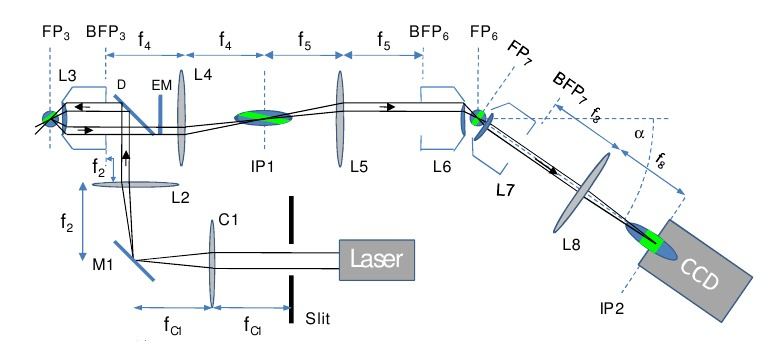
\includegraphics[width=12cm]{dunsby}
  \caption{Schematic of oblique plane microscopy (OPM). An index
    matched sample is excited using an oblique plane of light. The
    illuminated plane is tilted relative to the focal
    plane. Therefore, out-of-focus fluorophores on the periphery of
    the field of view are excited as well. Two additional objectives
    in the detection path are used to reconstruct an aberration free
    image of all the excited fluorophores (drawing from
    \cite{Dunsby2008}).}
  \label{fig:dunsby}
\end{figure}
Modern high numerical aperture objectives allow to illuminate an
\emph{index matched} sample with a half angle of up to
$70^\circ$. This enables illumination of an oblique and thin sheet of
light in the specimen just as in selective plane illumination
microscopy. However this technique (oblique plane microscopy, OPM) has
the advantage, that only one objective is used and therefore it will
work with conventional microscope slides. However, one difficulty is
that some of the excited fluorophores are severely defocused in the
intermediate image plane (plane IP1 in \figref{fig:dunsby}). Dunsby
describes how to rotate the observational plane optically in order to
recover an aplanatic image from the oblique illumination plane
\citep{Dunsby2008}. For this, they re-image the sample through two
additional objectives.

\nomenclature{OPM}{Oblique plane microscopy.}

\begin{figure}[!hbt]
  \centering
  \svginput{1}{hilo-sketch}
  \caption{Schematic of rays in HILO (highly inclined and laminated
    optical sheet) technique. The specimen is embedded in a medium of
    lower optical density than the immersion medium. For a very high
    illumination angle --- corresponding to a point on the periphery
    of the back focal plane --- the light would be reflected at the
    ``cover slip-medium'' interface due to total internal reflection
    (TIR). For HILO, a point on the back focal plane slightly closer
    to the optic axis is illuminated. The light enters the embedding
    medium at a highly inclined angle and only a thin sheet in the
    focal plane is illuminated \citep[inspired from][]{Tokunaga2008}.}
  \label{fig:hilo}
  % FIXME the construction of the rays is not correct, they should go
  % to the principal plane and then should be just axially shifted
  % into the aplanatic sphere.
\end{figure}


\nomenclature{TIR}{Total internatl reflection.}

Biological specimen are often not index matched and have a lower index
$n_e\approx 1.33\ldots1.45$ than the immersion oil $n=1.52$. As
indicated in \figref{fig:hilo}, the refraction at the interface
between cover slip glass and embedding medium can be exploited to
illuminate the specimen with a light sheet that is nearly parallel to
the focal plane.  This technique is called highly inclined and
laminated optical sheet microscopy (HILO) \citep{Tokunaga2008,
  Konopka2008}.

\nomenclature{HILO}{Technique for microscopy illumination: highly
  inclined and laminated optical sheet}

Note that the index mismatch between embedding and immersion medium
will introduce aberrations (mostly spherical) in the detection which
will limit the useful imaging depth to a few microns for high aperture
lenses.
\section{Scanning techniques with improved light utilization}
\begin{summary}
  A confocal microscope exposes out-of-focus fluorophores with
  approximately the same dose as the in-focus fluorophores when
  producing and image of a focal slice. During acquisition of z-stacks
  this results in bleaching and successive slice contain less and less
  signal. In particular living organisms may be harmed due to
  phototoxicity during the observation.

  Here I present two methods that can mitigate this effect. The first
  ist the two-photon microscop, in which the excitation is limited to
  the focal plane.

  Furthermore, there is controlled light exposure microscopy that
  selectively illuminates the sample depending on its structure. It
  delivers images with the overall quality as a conventional confocal
  while decreasing phototoxicity and bleaching considerably.

  This method is based on a feedback that controls excitation dose
  depending on the local fluorophore concentration and therefore
  benefits from any latency improvements. In this context I discuss
  two approaches that can increase the scanning speed considerably.
\end{summary}
\subsection{Two-photon laser scanning fluorescence microscopy}
\label{sec:2-photon}
If the laser intensity in the focal spot of a confocal microscope is
sufficiently high, then two infrared photons can be absorbed within
\unit[$\sim 5$]{fs} and excite the same electronic state.

In this regime, the fluorescence emission increases quadratically with
laser intensity \citep{goppert1931elementarakte}. This non-linearity
confines the excitation volume to the vincinity of the focal plane
\citep{Denk1990}. Fluorophores outside of this region are not
excited. Therefore this method produces sectioned images by default
and there is no need for a detection pinhole.

As an additional benefit infrared light is scattered less than visible
light of half the wavelength. This increases penetration depth and
image quality. Photodamage outside of the focal volume is unlikely and
phototoxicity is much lower, compared to the single-photon confocal
microscope, when $z-$stacks are acquired.

However, the phototoxicity within the focal volume is higher and
techniques like ultramicroscopy (section
\ref{sec:light-sheet-microscopy}) with single-photon excitation are
preferable, when low overall phototoxicity is a requirement.
\subsection{Controlled light exposure microscopy (CLEM)}
\label{sec:CLEM}
In the confocal microscope the excitation beam is scanned in a
rectangular grid over the focal plane. Normally this is done using two
galvanometer mirrors, one of which addresses pixel columns and the
other (much slower) addresses the rows. The excitation laser is
continuously active during a scan over one line. So ultimately, the
integration time at the detector defines horizontal sampling.
\begin{figure}[hbtp]
  \centering
  \svginput{1}{clem-sketch}
  \caption{ Schematic representation of a typical fluorescence image
    of a neuronal cell and histograms for three different regions. In
    the conventional confocal microscope areas without fluorophores
    (A) and the areas with many fluorophores (C) are subjected to an
    unnecessarily high light dose. Controlled light exposure
    microscopy (CLEM) adapts the illumination to the sample in order
    to reduce phototoxicity and bleaching.}
  \label{fig:clem}
\end{figure}

The measured signal in each pixel is proportional to the collected
photons and therefore subject to Poisson distributed quantum shot
noise (see section \ref{sec:photon-noise}). Thus, the signal-to-noise
radio fluctuates over the image. The image is particularly noisy in
areas with low fluorophore concentration. For the human observer and
many computer algorithms the noise in these particularly noisy areas
defines the image quality. The fact that areas with more signal have
considerably less noise does not increase the perceived image quality,
neither does it improve the results of an edge detector for the dim
areas. Considering the detrimental effects of the excitation light it
would be advantageous to acquire fluorescence images with constant
signal-to-noise ratio in each pixel.



This approach is pursued in the controlled light exposure microscope
(CLEM). It utilizes a confocal microscope, adapted for fast switching
of the excitation light. Depending on whether the photons collected
during a short preparation time, each pixel is classified into one of
three classes. The darkest pixels (class A in \figref{fig:clem}) are
assumed to not contain any information and the laser is switched off
for the remainder of the dwell-time. Pixels with moderately many
photons (class B) are illuminated for the entire dwell-time. For
pixels with a high fluorophore concentration (class A) the excitation
laser is turned off, once a certain number of photons have been
detected. In this case the signal is not the number of photons but the
illumination duration.

In this way, one obtains a picture in which bright regions have a
constant signal-to-noise ratio and regions without fluorophores are
illuminated with only a small dose. Especially when capturing z-stacks
this procedure significantly reduces phototoxicity and photobleaching
--- with an insignificant decline in image quality.

%  Unfortunately, due to the photon nature of
% light, sometimes a region of type (B) is incorrectly classified as (A)
% which introduces dark pixel artifacts in the image \citep{Hoebe2010}.

The CLEM approach was first presented by Hoebe et al.\ in 2007,
followed by an independent similar version with adaptive control of
the laser power for 2-photon microscopy by Chu et al.\
\citep{Hoebe2007,Chu2007}.

% FIXME i'm not sure if 2007 was first publication
\subsection{Fast beam steering}
In a conventional confocal microscope, the beam is steered by two
galvanometer mirrors. While this technique offers very good light
throughput the inertia of the mirrors limit the access rate of spots
in the focal plane. The CLEM technique could be simplified and
improved by an inertia-free solution to steer the excitation beam from
pixel to pixel. The laser intensity would no longer have to be
modulated and when enough photons were collected in a pixel, the next
one could be addressed.

The z-focus is often controlled by piezomechanical elements that
either move the sample or the objective, i.e.\ objects of relatively
large mass. Therefore, the settling time for focus movements has a
correspondingly large latency and focusing is often much slower than
lateral pixel access.

\subsubsection{Acousto-optic deflectors for fast beam steering}
An interesting alternative to galvanometric mirrors are acousto
optical deflectors (AODs). They consist of a transparent optical
element into which an acoustic wave is coupled by means of an
ultrasound transducer.  An acoustic wave is a longitudinal variation
of the interatomic distance and thereby affects the local electron
density and thus the refractive index of the medium. An acoustic wave
in an AOD allows to diffract a beam of light with moderate efficiency
(70\%). Changing the acoustic frequency allows to vary the angle of
diffraction. Due to its strong chromatic aberration and low
efficiency, an AOD should not be used to descan the beam of a normal
confocal microscope. However, this device is well suited for a
two-photon microscope, where descanning is not strictly necessary.  In
\cite{Otsu2008} the authors achieved a switching time of $\unit[4]{\mu
  s}$ using an acoustic wave in tellurium dioxide (TeO$_2$).

\begin{figure}[htbp]
  \centering
  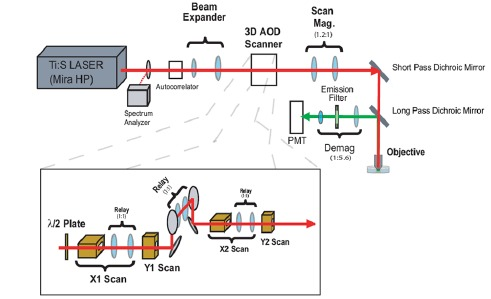
\includegraphics[width=12cm]{aod} 
  \caption{Schematic of an acousto-optic deflector (AOD) illumination
     system with $z-$focusing. Figure taken from \citet{Reddy2008}}
% in focusing single s highly preferred http://www.future-perfect.co.uk/grammartips/grammar-tip-focussed-focused.asp
  \label{fig:aod}
\end{figure}

\nomenclature{AOD}{Acousto-optic deflector}
\nomenclature{AOM}{Acousto-optic modulator}

The system in \cite{Reddy2008} even uses an acousto optic technique to
focus the excitation beam of a two-photon microscope. The authors
exploit the fact that the excitation light consists of laser
pulses. The ultrasound transducer is synchronized to the laser pulses
and generates an acoustic waveform that resembles an one-dimensional
Fresnel zone --- high frequencies on the outside and low frequencies
towards the center. The synchronization ensures that each pulse
encounters a diffraction grating that is symmetric with regards to the
optical axis. Two such elements in a row but rotated by 90 degrees
allow to focus the beam, similar to how two cylindrical lenses would
(see \figref{fig:aod}).

\subsubsection{Aberration-free optical refocusing}
Achieving the resolution limit of modern microscope objectives using
acousto-optic Fresnel zones seems impossible or at least very
difficult. An alternative approach that can significantly speed up
conventional focusing techniques is based on a similar technique as
the oblique plane microscope (see section \ref{sec:hilo}). In
\cite{Botcherby2007} and \cite{botcherby2012aberration} an additional
objective produces an unmagnified three-dimensional image of the
sample which allows rapid refocusing with a lightweight mirror. This
approach is achromatic and allows to focus many tens of microns deep
into the sample while maintaining diffraction limited
resolution. Unlike the acousto-optic device this method is not limited
to a single collimated beam and can be applied in widefield
microscopes.

\section{Non-scanning techniques}
\subsection{Intensity modulation}
\subsubsection{Programmable array microscopy}
\label{ref:pam}
The main element of the programmable array microscope is a digital
micromirror (DMD). It is placed into the intermediate image and acts
simultaneously in the excitation as well as the detection beam
path. The mirrors can be programmed to have one of two
deflections. Either they send light into the sample or they send it
into a beam dump. This allows structured illumination with a
computationally defined pattern. In the simplest case, when only a
single pixel is turned on, the operation of the PAM resembles that of
a confocal microscope. Fluorescence light of in-focus fluorophores
returns to the micromirror that was responsible for the excitation and
is directed towards the camera~1. Out-of-focus fluorescence will be
reflected by any of the other DMD mirrors and ends up on camera 2.

\begin{figure}[htbp]
  \centering
  \svginput{1}{pam-sketch}
  \caption{Schematic of a programmable array microscope (PAM)
    \citep[inspired from][]{Verveer1998}. A digital micromirror
    device (DMD) containing an array of tiltable mirrors is imaged
    into the focal plane of the objective. Returning fluorescent light
    from out-of-focus fluorophores is distributed onto both the
    cameras. In-focus fluorescence is only imaged onto camera 1.}
  \label{fig:pam-sketch}
\end{figure}


At the time when \cite{Heintzmann2001a} was written, EM-CCDs were not
widely available. In order to reduce the effects of readout noise,
cameras~1 and 2 integrate for a long time while the DMD displays many
patterns. The pattern sequence could for example be a single pixel
which scans the entire field. This would be very slow, so instead,
patterns of a pseudorandom sequence are presented which significantly
accelerates data acquisition because each individual pattern excites
more in-focus information. However, at the same time crosstalk is
increased, i.e.\ additional light from out-of-focus fluorophores is
collected on camera 1.  The images from both cameras for z-stack
acquisitions are reconstructed using a maximum likelihood
deconvolution.

A technique similar to controlled light exposure microscopy (CLEM,
section \ref{sec:CLEM}) has been implemented in a programmable array
microscope (PAM) \citep{Caarls2011}. 


There are a few drawbacks with the programmable array microscope:
First, diffraction losses at the DMD reduce detection
efficiency. Second, if excitation light causes fluorescence or Raman
scattering at the DMD surface, it is impossible to distinguish this
disturbance from the fluorescence signal of the sample. Third, it is
difficult to align the optics such that DMD pixels are imaged exactly
and without distortion on camera pixels.

Distorted imaging could be retrospectively corrected by
interpolation. However, this process would destroy the known noise
characteristics of the sample values. The values in an interpolated
image are no longer Poisson distributed and application of the maximum
likelihood estimation is problematic.

With the availability of cameras with sub-electron readout noise
(EM-CCD or sCMOS) one would no longer place the DMD in the detection
path. Instead, one could acquire an image of each individual pattern
and do the descanning computationally.


\nomenclature{PAM}{Programmable array microscopy}%
\nomenclature{DMD}{Digital micro mirror device}%
\nomenclature{MLE-PAM}{Minimized light exposure programmable array microscope}%
\subsection{Direct illumination}
An obvious method for doing spatial control is to image a
two-dimensional array of high-power micro-LEDs into the specimen.
\begin{figure}[hbtp]
  \centering
  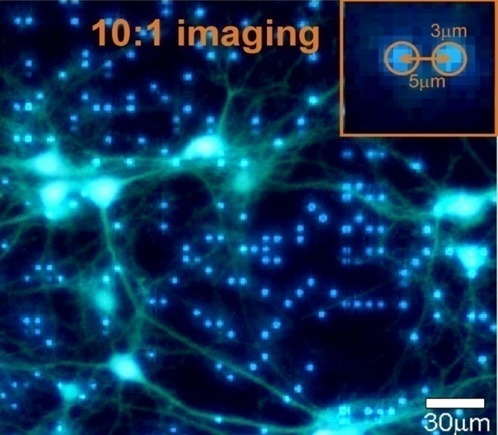
\includegraphics[width=7cm]{led-array} 
  \caption{An overlay combining wide field micro-LED illumination and
    fluorescence imaging YFP tag expressed in neurons, taken from
    \citet{grossman2010}.}
  \label{fig:led-array}
\end{figure}
However, the problem is to achieve sufficient \emph{irradiance} and
\emph{fill factor}. The angular emission profile of LEDs is often
Lambertian, i.e.\ the back focal plane of the objective would be
over-illuminated and a lot of light would be lost. The fill factor is
limited because it is difficult to put a lot of LEDs close to each
other.  The technique has been demonstrated using a $64\times64$ array
of $\unit[20]{\mu m}$ micro-emitters with $\unit[50]{\mu m}$ pitch
\citep{grossman2010}.  The LEDs can be switched at millisecond speed
and emit at a wavelength of $\unit[(470\pm22)]{nm}$.

\nomenclature{GFP}{Green fluorescent protein}
\nomenclature{EGFP}{Enhanced green fluorescent protein}
\nomenclature{YFP}{Yellow fluorescent protein}
\nomenclature{VCSEL}{Vertical-cavity surface-emitting laser}
\nomenclature{LED}{Light emitting diode} % Fixme
\nomenclature{MMA}{Micromirror array}
\nomenclature{LCoS}{Liquid crystal on silicon (display)}
\nomenclature{DPSS}{Diode-pumped solid-state (laser)}

Currently it is not clear whether direct illumination will ever
replace the more flexible spatial light modulators. Manufacturers of
direct illumination devices will optimize their technology for
consumer applications such as mobile phone displays where neither fill
factor nor extreme radiant intensity (\unit[]{W/sr}) are very
important.  Arrays of Vertical-cavity surface-emitting lasers (VCSEL)
may become interesting alternatives to LED-arrays because they can
provide high radiant intensity but currently they are not readily
available in the interesting wavelength ranges.


\subsubsection{Light field microscopy}
\label{sec:light-field-microscopy}
Interesting work on light fields originally started in the macroscopic
domain of cameras \citep{Lippmann1908 %,Sokolov1911 % I'm sorry but I can't cite russian. Can't figure out how to make it work in tex
} and was eventually
applied as a technique for microscopy
\citep{Levoy2006,Levoy2009,Zhang2009}. This approach is built on
imaging through an array of microlenses.
\begin{figure}[!hbt]
  \centering
  %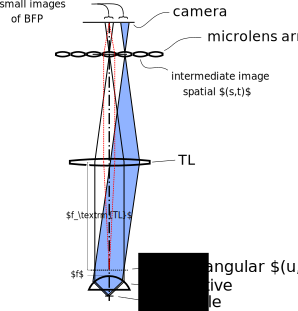
\includegraphics[width=7cm]{microlens-levoy-sketch} %FIXME redraw
  \svginput{1}{microlens-levoy-sketch}
  \caption{Schematic of microlenses in the intermediate image plane
    \citep[inspired from][]{Levoy2006}. A spatial intensity modulator
    is illuminated from the right with an extended light
    source. Groups of neighboring pixels downstream of individual
    microlenses are imaged into the pupil. Therefore these pixels
    allow to control the irradiance in the sample at the area that is
    conjugated to the microlens. }
  \label{fig:microlens-levoy-sketch}
\end{figure}


Downstream of the microlenses a spatial light modulator (SLM) is
placed, so that a rectangular group, of say $10\times 10$ pixels is
imaged into the pupil. Each microlens illuminates the pupil from
another angle. In \cite{Levoy2009} they use an intensity SLM and each
of its pixels controls the radiant intensity (\unit[]{W/sr}) in the
area of the sample that is covered by the conjugated image of the
corresponding microlens. A trade-off has to be made between the
resolution that can be obtained in the pupil and the resolution in the
focal plane in the sample. The latter is limited by the size of the
microlenses.

The paper uses microlenses in the detection path as well. The camera
captures a lot of images of the pupil. This allows retrospective
refocusing or rotation of the image using the ray-based plenoptic
theory. However, splitting the images with microlenses has severe
drawbacks and should not be used with fluorescence microscopy. When
recording camera images, important phase information is lost and the
sub-images can not be recombined to obtain the full resolution of the
microscope objective.

In the case of illumination the loss in resolution is not as important
and perhaps the full resolution could even be maintained when a phase
SLM is used.
\nomenclature{TL}{tube lens}
\subsection{Temporal focusing}
\begin{figure}[!hbt]
  \centering
  \svginput{1}{temporal-focus-sketch}
  \caption{Schematic of temporal focusing \citep[inspired
    from][]{Oron2005}. A grating in the intermediate image plane
    separates the pulse into its spectral components. The out-of-focus
    areas of the specimen are illuminated with a longer pulse. Only in
    the focal plane, all spectral components interfere coherently and
    form a short intensive pulse.}
  \label{fig:oron}
\end{figure}
The axial extent of ultra-short laser pulses can be as thin as a few
microns. A parallel beam can be split into different spectral
components by a grating in the intermediate image plane
\citep{Oron2005}. The tube lens focuses the diffraction pattern into a
line in the back focal plane of the objective.

The objective, which has to be corrected for chromatic aberration and
dispersion, then focuses all the beams onto the focal plane. Different
spectral components arrive in the focal plane at the same time. The
out-of-focus points see an extended illumination. For a high NA
objective, a pulse duration of $\tau=\unit[20]{fs}$ results in slice
of $z\approx\tau c/2\approx\unit[3]{\mu m}$ thickness around the
focus, where the beam has significant intensity.

Using this technique it is possible to build a wide field 2-photon
microscope that only excites fluorophores within the focal plane. The
technique can be further improved by spatially modulating the beam in
the intermediate image plane for CLEM like performance. This technique
has been implemented in the TF-GPC approach and will be discussed in
the next section.

\subsection{Phase modulation}
\subsubsection{Digital holography}
\begin{figure}[!hbt]
  \centering
  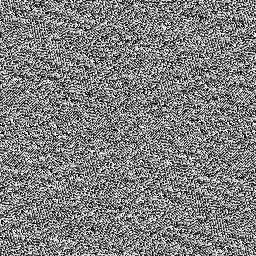
\includegraphics{myholo}\quad
  \svginput{1}{phase-holo_my} 
  \caption{Schematic of spatial illumination by phase holography. A
    phase-only SLM displays a hologram in the plane $P'$ which is
    conjugated to the back focal plane $P$ of the objective
    \citetext{inspired by slide from V. Emiliani}.}
  \label{fig:phase-holo}
\end{figure}
Certain types of liquid crystal spatial light modulators can be used
to modify the phase of light. When such a device is placed into the
back focal plane of a lens, it is possible to control the light
distribution in its front focal plane. An iterative algorithm
(iterative Fourier transform algorithm, IFTA) can be used to establish
a phase image on the liquid crystal display that will result in an
intensity distribution in front of the lens.

\nomenclature{IFTA}{Iterative Fourier transform algorithm}

This approach has been used to excite a two-dimensional pattern in the
specimen \citep{Lutz2008,Zahid2010} and is advantageous especially for
cases where only small parts of the specimen ought to be
illuminated. As opposed to conventional intensity spatial light
modulators, the light can be redirected from dark areas into the
bright areas.

% single photon 405nm uncaging, ifta,
% spherical wave approximation
There is also a limited possibility to create three-dimensional
patterns, e.g.\ several points below, in and above the focal plane by
displaying Fresnel zone planes.  For illumination, usually a laser
with non-zero interference length is employed. However, this
illumination contains an unwanted ``speckle'' pattern in the form of
noisy non-uniformities. To a certain extent, the contrast of the
speckle pattern can be reduced by controlling spatial and temporal
coherence of the illumination (sweeping the frequency of the laser or
changing illumination direction while the detector is integrating).

Holographic control can be used with 2-photon excitation as well
\citep{Nikolenko2008}, % two photon
but this exacerbates the effect of speckles.
\subsubsection{Generalized phase contrast (GPC)}
\begin{figure}[!hbt]
  \centering
  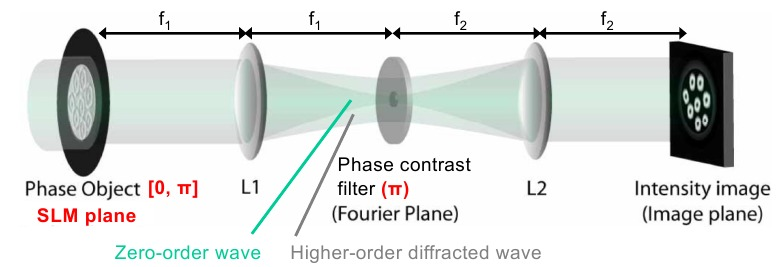
\includegraphics[width=14cm]{phase} % FIXME redraw
  \caption{Schematic of generalized phase contrast
    \citep[from][]{Rodrigo2008}.}
  \label{fig:phase}
\end{figure}
A phase contrast microscope objective \todo{modified ?} can be used to
convert a phase image from the intermediate image plane into an
intensity image in the specimen \citep{Rodrigo2008}\todo{read more of
  this}. Compared to digital holography, hardly any computation is
necessary. Yet, the phase spatial light modulator allows to
concentrate a lot of light even on a small region of the specimen as
opposed to other techniques, which involve intensity modulation and
lose all the light of dark areas by sending it into a beam block or
something similar.

The generalized phase contrast method is suitable even with spatially
incoherent illumination\todo{slightly ?}. However, when the
fill-factor -- the size of the bright area in the image -- changes,
the phase contrast filter must be changed.
\subsubsection{Generalized phase contrast and temporal focusing (TF-GPC)}
The combination of generalized phase contrast and temporal focusing
allows spatially controlled illumination of in-focus areas
\citep{Papagiakoumou2010}. Usage of a phase spatial light modulator
results in high light efficiency compared to intensity modulation.
Splitting and recombination of the spectral components of the pulse
reduce speckle noise considerably.
\begin{figure}[!hbt]
  \centering
  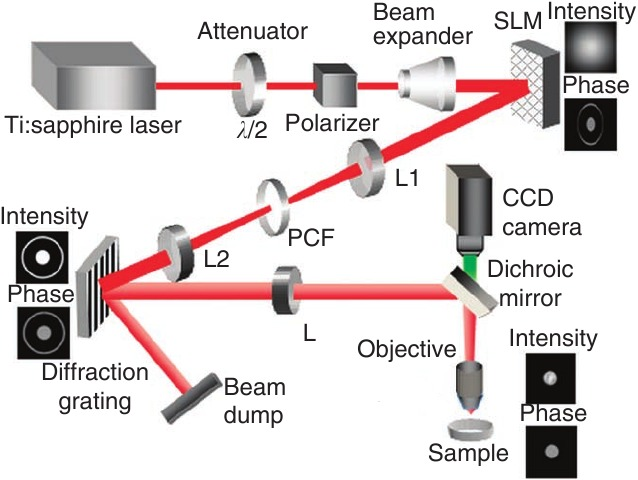
\includegraphics[width=11cm]{tf-gpc} 
  \caption{Schematic of phase contrast with temporal focusing (TF-GPC)
    \citep[from][]{Papagiakoumou2010}, PCF is a phase contrast filter.}
  \label{fig:tf-gpc}
\end{figure}
\nomenclature{PCF}{Phase contrast filter}

%%% Local Variables: 
%%% mode: latex
%%% TeX-master: "kielhorn_memi"
%%% End: 
